\section{FreshQA Public Main And Sequence: Volatile Public Boundary}

The official FreshQA public runs are the paper's clearest boundary evidence. They evaluate the same controller on frozen public changing-answer data derived from weekly releases, once on a changed-question-heavy main slice and once on a sequence slice with repeated corrections and forgetting probes. Across all four official models, retrieval dominates.

\begin{table}[h]
\centering
\small
\begin{tabular}{llrrrrr}
\toprule
Model & Policy & Quality & 95\% CI & Retrieve & Adapt & Stale \\
\midrule
FLAN-T5 Base & Retrieval only & 1.000 & [1.000, 1.000] & 796.0 & 0.0 & 0.000 \\
FLAN-T5 Base & Retrieve gate & 0.132 & [0.132, 0.132] & 89.0 & 0.0 & 0.005 \\
FLAN-T5 Base & Full router & 0.616 & [0.544, 0.687] & 448.6 & 69.8 & 0.002 \\
FLAN-T5 Base & Calibrated router & 0.694 & [0.634, 0.754] & 528.4 & 18.0 & 0.001 \\
FLAN-T5 Base & Router without delayed utility & 0.985 & [0.985, 0.985] & 740.0 & 4.0 & 0.000 \\
FLAN-T5 Small & Retrieval only & 1.000 & [1.000, 1.000] & 796.0 & 0.0 & 0.000 \\
FLAN-T5 Small & Retrieve gate & 0.134 & [0.134, 0.134] & 89.0 & 0.0 & 0.003 \\
FLAN-T5 Small & Full router & 0.612 & [0.539, 0.684] & 448.6 & 69.8 & 0.001 \\
FLAN-T5 Small & Calibrated router & 0.794 & [0.725, 0.863] & 612.4 & 29.4 & 0.000 \\
FLAN-T5 Small & Router without delayed utility & 0.984 & [0.984, 0.984] & 739.0 & 4.0 & 0.000 \\
\bottomrule
\end{tabular}

\caption{Official FreshQA public main results on the primary FLAN matrix. Retrieval is perfect; calibration partially repairs the full router, but \texttt{router\_no\_v\_future} remains much closer to the retrieval ceiling.}
\label{tab:freshqa-main}
\end{table}

On the public main slice, \texttt{always\_retrieve} is 1.000 on both FLAN backbones. The full router falls to 0.616 on FLAN-T5-Base and 0.612 on FLAN-T5-Small. Calibration helps on this slice, reaching 0.694 and 0.794, but \texttt{router\_no\_v\_future} is still much stronger at 0.985 and 0.984. The paired sign tests are decisive: retrieval beats the full router, the calibrated router, and \texttt{router\_no\_v\_future} on both FLAN models, while \texttt{router\_no\_v\_future} significantly outperforms both router variants.

\begin{figure}[h]
\centering
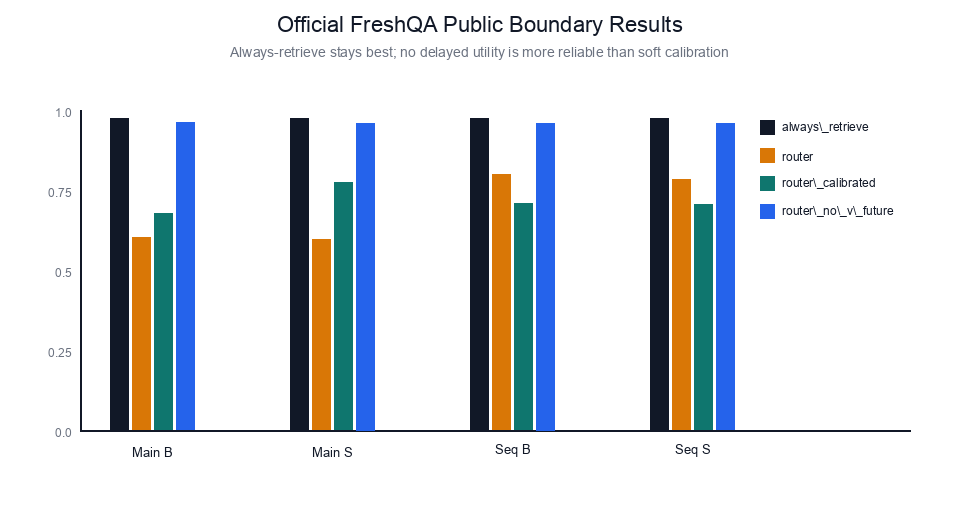
\includegraphics[width=0.95\linewidth]{../shared/generated/word_assets/fig_public_main_calibration_curve.png}
\caption{Official public-boundary comparison on the primary FLAN matrix. Retrieval is perfect on both FreshQA public slices, while \texttt{router\_no\_v\_future} stays much closer to that ceiling than the full or calibrated router.}
\label{fig:public-best-mode}
\end{figure}

\begin{table}[h]
\centering
\small
\begin{tabular}{llrrrrr}
\toprule
Model & Policy & Quality & 95\% CI & Retrieve & Adapt & Stale \\
\midrule
FLAN-T5 Base & Retrieval only & 1.000 & [1.000, 1.000] & 796.0 & 0.0 & 0.000 \\
FLAN-T5 Base & Retrieve gate & 0.132 & [0.132, 0.132] & 89.0 & 0.0 & 0.005 \\
FLAN-T5 Base & Full router & 0.819 & [0.708, 0.930] & 630.0 & 84.6 & 0.000 \\
FLAN-T5 Base & Calibrated router & 0.725 & [0.647, 0.804] & 540.6 & 26.4 & 0.000 \\
FLAN-T5 Base & Router without delayed utility & 0.984 & [0.984, 0.984] & 739.0 & 5.0 & 0.000 \\
FLAN-T5 Small & Retrieval only & 1.000 & [1.000, 1.000] & 796.0 & 0.0 & 0.000 \\
FLAN-T5 Small & Retrieve gate & 0.134 & [0.134, 0.134] & 89.0 & 0.0 & 0.003 \\
FLAN-T5 Small & Full router & 0.802 & [0.687, 0.916] & 614.0 & 82.0 & 0.000 \\
FLAN-T5 Small & Calibrated router & 0.724 & [0.643, 0.804] & 539.2 & 26.6 & 0.000 \\
FLAN-T5 Small & Router without delayed utility & 0.982 & [0.982, 0.982] & 738.0 & 5.0 & 0.000 \\
\bottomrule
\end{tabular}

\caption{Official FreshQA public sequence results on the primary FLAN matrix. On repeated correction chains, suppressing delayed utility is again much safer than the full router, and soft calibration is inconsistent.}
\label{tab:freshqa-sequence}
\end{table}

The sequence slice makes the boundary even clearer. Retrieval again stays at 1.000. The full router reaches 0.819 on FLAN-T5-Base and 0.802 on FLAN-T5-Small, while calibration is actually worse on both primary models at 0.725 and 0.724. \texttt{Router\_no\_v\_future} again stays much closer to retrieval at 0.984 and 0.982, and the corresponding sign tests show it significantly outperforming both router variants. Cross-family robustness in the appendix shows the same qualitative pattern on Qwen2.5-1.5B and SmolLM2.

\begin{table}[h]
\centering
\small
\begin{tabular}{lr}
\toprule
Audit field & Count \\
\midrule
Always-retrieve correct / router wrong & 40 \\
Always-retrieve correct / calibrated-router wrong & 25 \\
Alias-heavy or multi-answer & 20 \\
Rollback / forgetting / answer-change probes & 15 \\
\midrule
Clean verdicts & 24 \\
Suspect verdicts & 76 \\
Leakage-risk verdicts & 0 \\
\bottomrule
\end{tabular}

\caption{Official FreshQA manual audit summary. The audit found no direct leakage-risk cases, but many cases remain suspect, so the public trust story is bounded rather than fully cleared.}
\label{tab:freshqa-audit}
\end{table}

The manual audit is important for interpretation. Among 100 audited cases, 24 were labeled clean, 76 were labeled suspect, and none were labeled direct leakage risk. That is enough to reject a simple leakage explanation for the retrieval-dominant result, but not enough to treat the benchmark as perfectly trust-cleared. The right conclusion is modest: public changing-answer evaluation is hard, retrieval is the safest policy in our current setup, and delayed utility should usually be suppressed rather than softly calibrated in this regime.
